\documentclass[12pt]{article}
\usepackage[a4paper, margin=2cm]{geometry}
\usepackage[english]{babel} % To obtain English text with the blindtext package
\usepackage{blindtext}
\usepackage{graphicx} % Required for inserting images
\usepackage{array} % For extra column formatting
\usepackage{amsmath} %for equation environment
\usepackage{float}
\usepackage{parskip} % For gaps between para
\usepackage{setspace}
\usepackage{pdfpages}
\usepackage{abstract}
\usepackage[export]{adjustbox}
\usepackage{emptypage}
\usepackage{tocloft}
\usepackage[nottoc]{tocbibind}
\usepackage{hyperref, url}
\usepackage{subcaption}
\usepackage{lipsum}
\usepackage{xcolor}


\cftsetindents{section}{0em}{2em}
\cftsetindents{subsection}{0em}{2em}

\renewcommand\cfttoctitlefont{\hfill\Large\bfseries}
\renewcommand\cftaftertoctitle{\hfill\mbox{}}

\graphicspath{ {./images/} }

\pagenumbering{arabic}

\definecolor{blurple}{HTML}{5865F2}

\hypersetup{
    colorlinks=true,
    linkcolor=black,
    urlcolor=blurple,
    citecolor=blurple,
}

\urlstyle{same}
%%%%%%%%%%%%%%%%%%%%%%%%%%%%%%%%%%%


\title{PHYC20040 Exp.1 Hubble RS}
\author{Joana Adao}
\date{\today}

\begin{document}

\begin{titlepage}
    \begin{center}

        \begin{figure}[ht]
            
\includegraphics[width=\textwidth]{UCDLogo.png}
        \end{figure}
        
        \begin{figure}
            \centerline{
\includegraphics[width=\paperwidth]{UCDBanner.png}}
        \end{figure}

        \vspace{4cm}

        {\LARGE \bfseries PHYC20040 Exploring the Solar System}\\
        \vspace{0.75cm}
        {\Large Experiment No.1 Hubble Redshift Distance Relation}
        
        \vspace{1cm}
    
    {\Large \textbf{29 January 2025 }}

    \vspace{2cm}
    
    {\large \textbf{by Joana C.C. Adao (Student No. 23311051)}}\\

    \end{center}
    
   \clearpage

\end{titlepage}

\setcounter{page}{1}
\tableofcontents

\newpage

\begin{abstract}
\addcontentsline{toc}{section}{Abstract}

The aim of this experiment was to



\end{abstract}


%%%%%%%%%%%%%%%%%%%%%%%%%%%%%%%%%%%


\section{Theory}

\subsection{Brief History} \label{sec:1.1}

\subsubsection{The "Big Bang" Theory} \label{sec:1.1.1}

The "Big-Bang" theory is the most widely accepted explanation about the creation and \allowbreak expansion of the universe to date
\cite{britbigbang,spacebigbang}.
The theory states that, about 13.8 billion years ago, the universe began as simply an incredibly hot, such that atoms did not exist, 
and dense point of matter
\cite{britbigbang,spacebigbang,hubblebigbang}.
As the universe rapidly expanded the temperature and density decreased significantly
\cite{britbigbang,hubblebigbang}.
As the universe cooled certain nuclei came into existence. The theory suggests definite amounts of helium, hydrogen, and lithium were produced at this time
\cite{britbigbang}.

\begin{figure}[H]
    \centering
    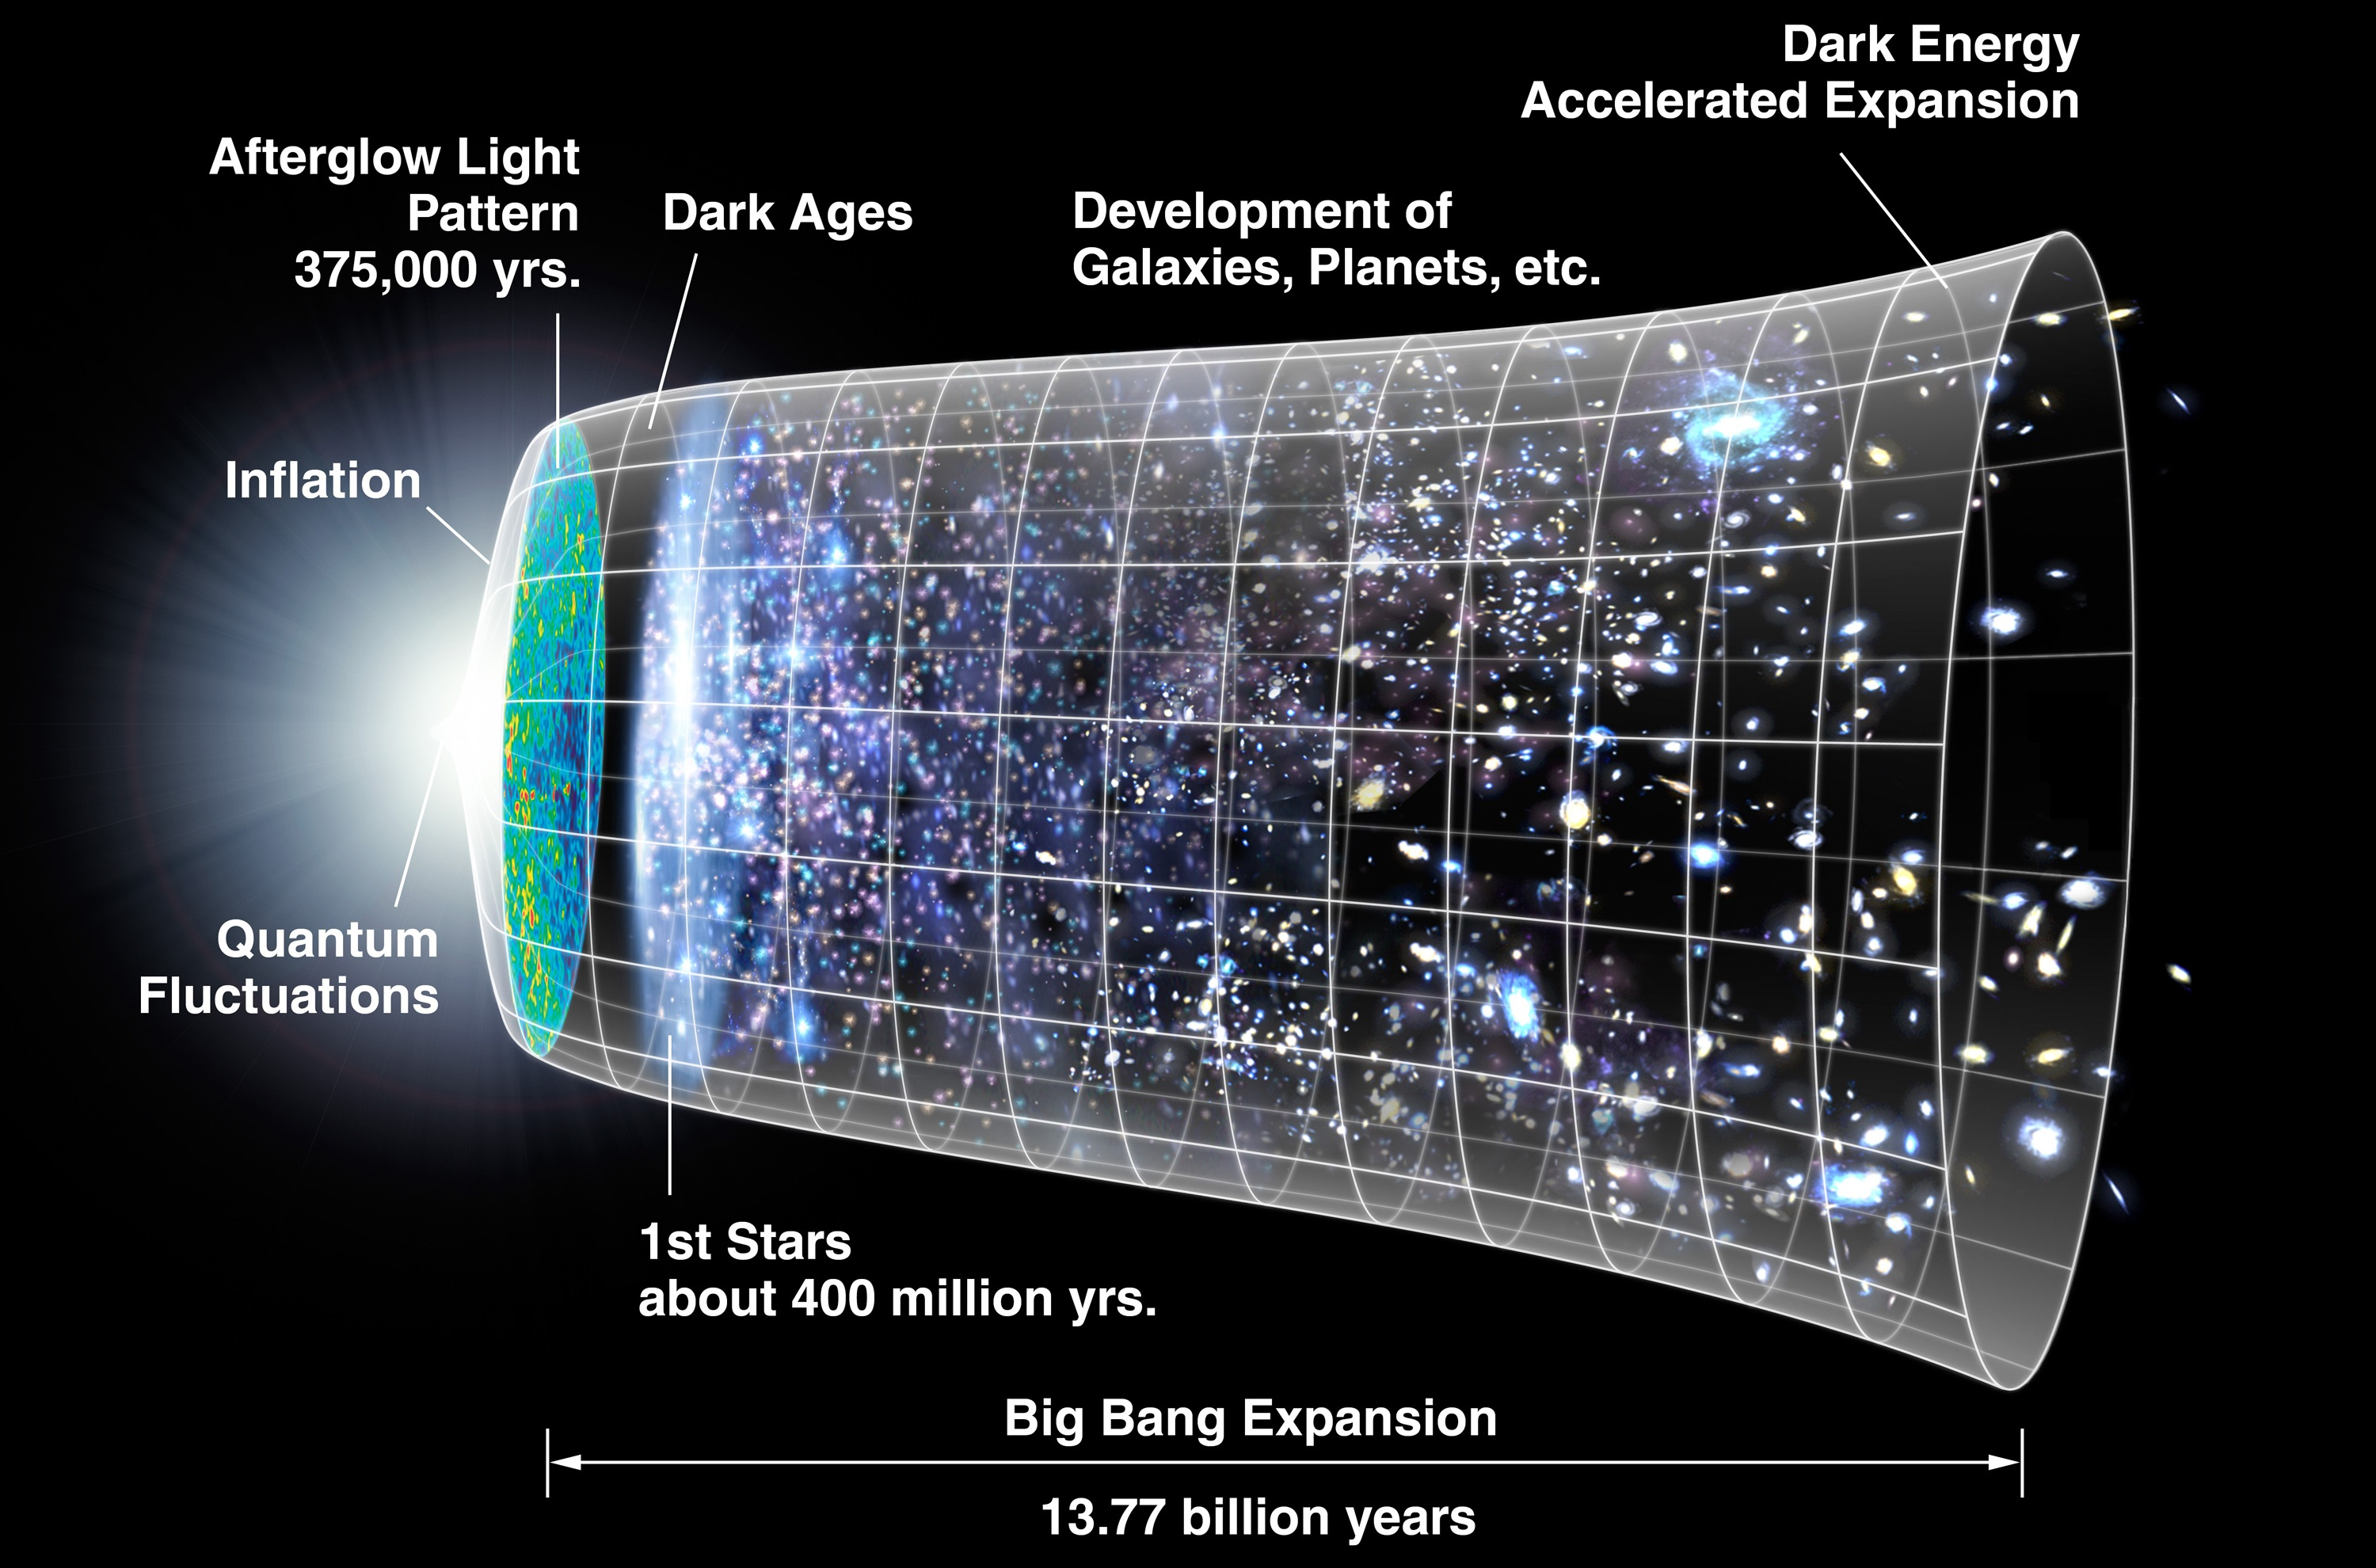
\includegraphics[width=15cm]{bigbang.jpg}
    \caption{\centering \footnotesize{Timeline of the Expansion of the Universe as per the Big Bang Theory (\textit{Time and Size not to Scale})} \protect\cite{bigbangpic}}
    \label{fig:bigbang}
\end{figure}

Matter, some atoms, formed \cite{hubblebigbang} and dominated over the antimatter \cite{britbigbang}.
Under the assumption that Albert Einstein's general theory of relativity correctly describes the relationship between matter and gravitational forces,
gravity brought matter into greater clumps that are known in the current day as our stars, planets, and galaxies
\cite{hubblebigbang}.

With the rapid expansion, the universe released a flood of radiation, alongside the matter, was also released into the new vast space
\cite{britbigbang,spacebigbang}
in the process known as "reheating", which is "the process whereby the inflation's energy density is converted back
into conventional matter after inflation
\cite{reheating}.
The radiation that was released then travelled through space, and the remnants of the early stages of the universe are known
as the cosmic microwave background (CMB) radiation \cite{britbigbang}, seen in figure \ref{fig:cmb}, 
though sometimes also referred to as the "'afterglow' of the Big Bang"
\cite{spacebigbang}.
These measurments are what allow scientists to predict the age of the universe relative to the currently measured rate of expansion of the universe
\cite{hubblebigbang}

\begin{figure} [H]
    \centering
    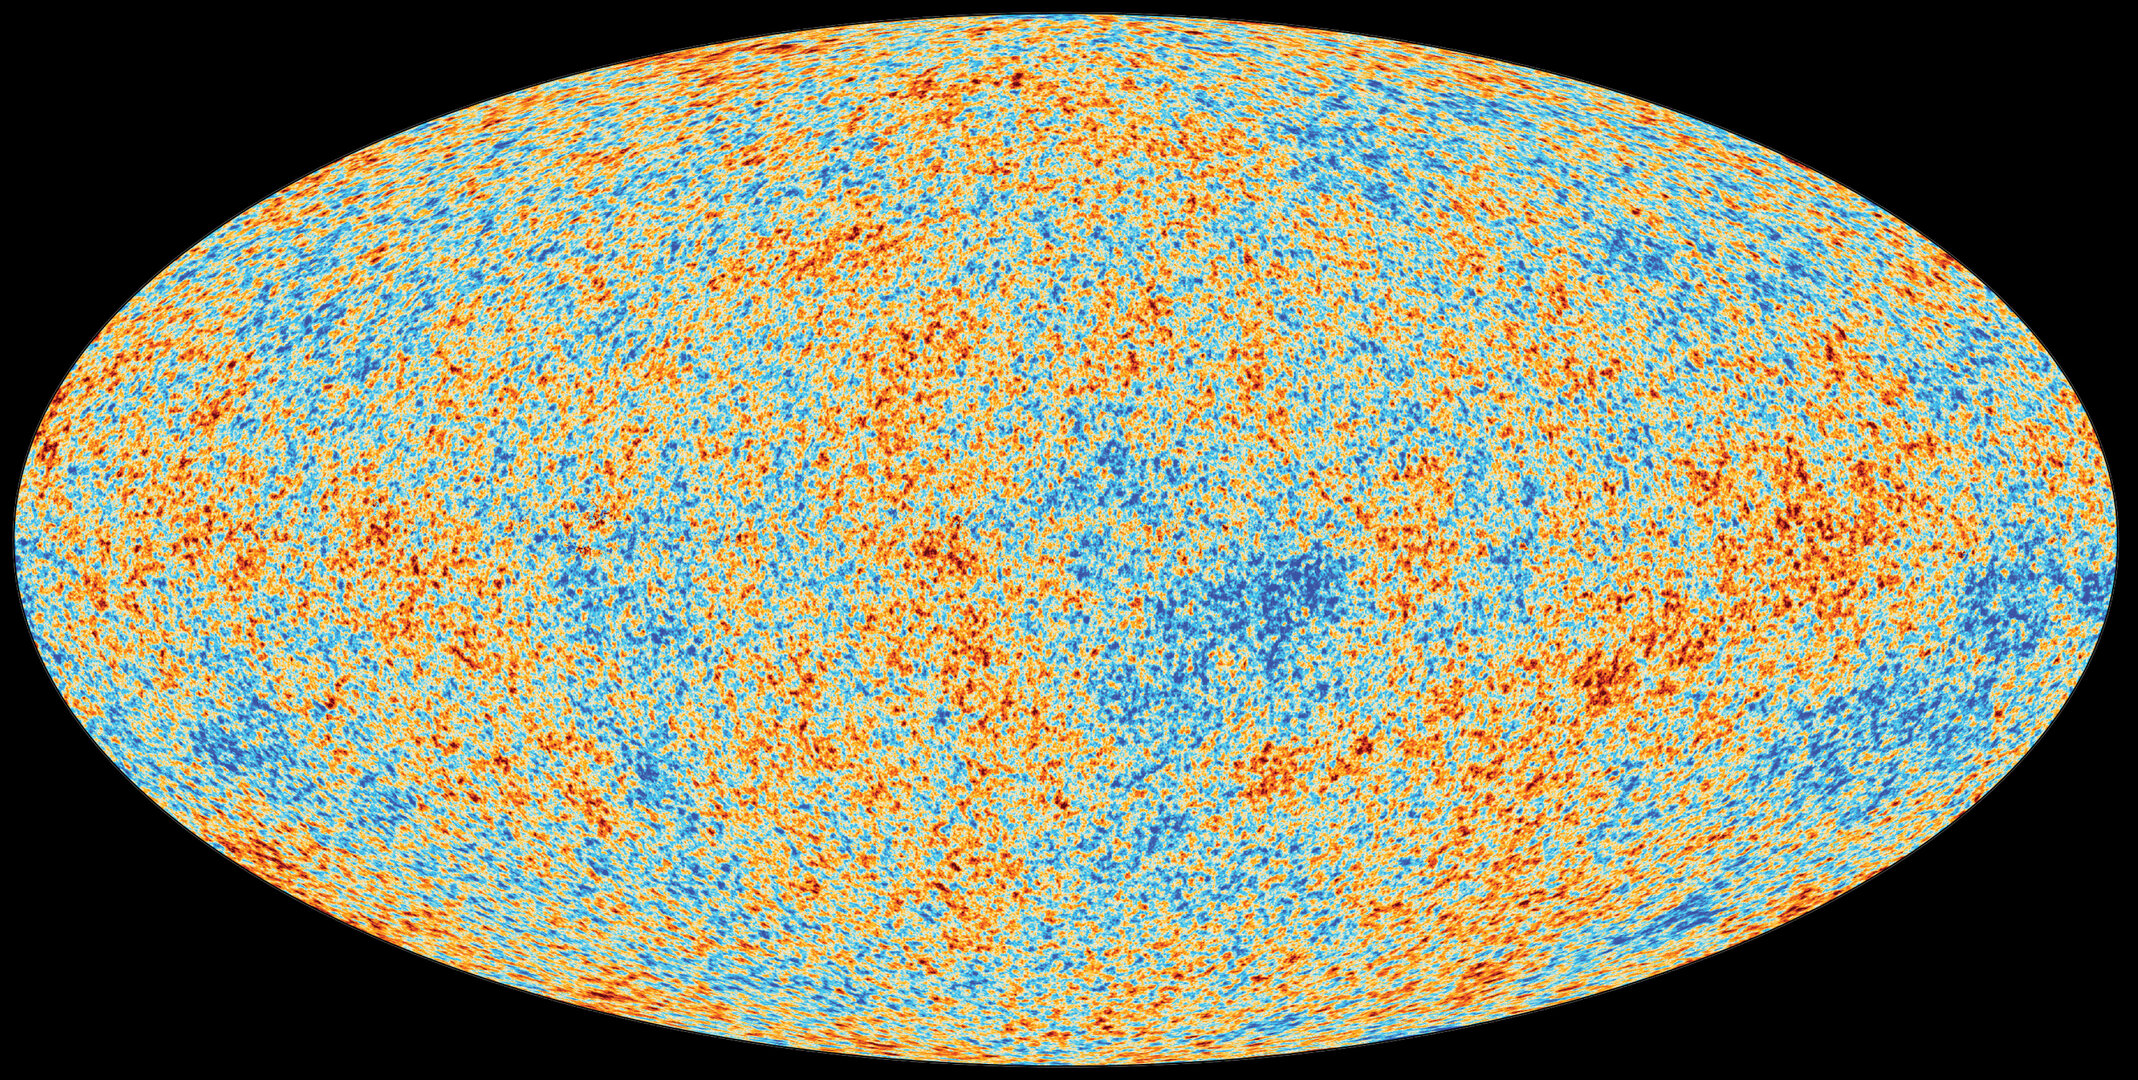
\includegraphics[width=\textwidth]{cmb.jpg}
    \caption{\centering \footnotesize{Cosmic Microwave Background (CMB) Radiation \protect\cite{cmbpic}}}
    \label{fig:cmb}
\end{figure}

\subsection{Spectrum, Spectrometry, Spectrograph} \label{sec:1.2}



\begin{figure}[H]
    \centering
    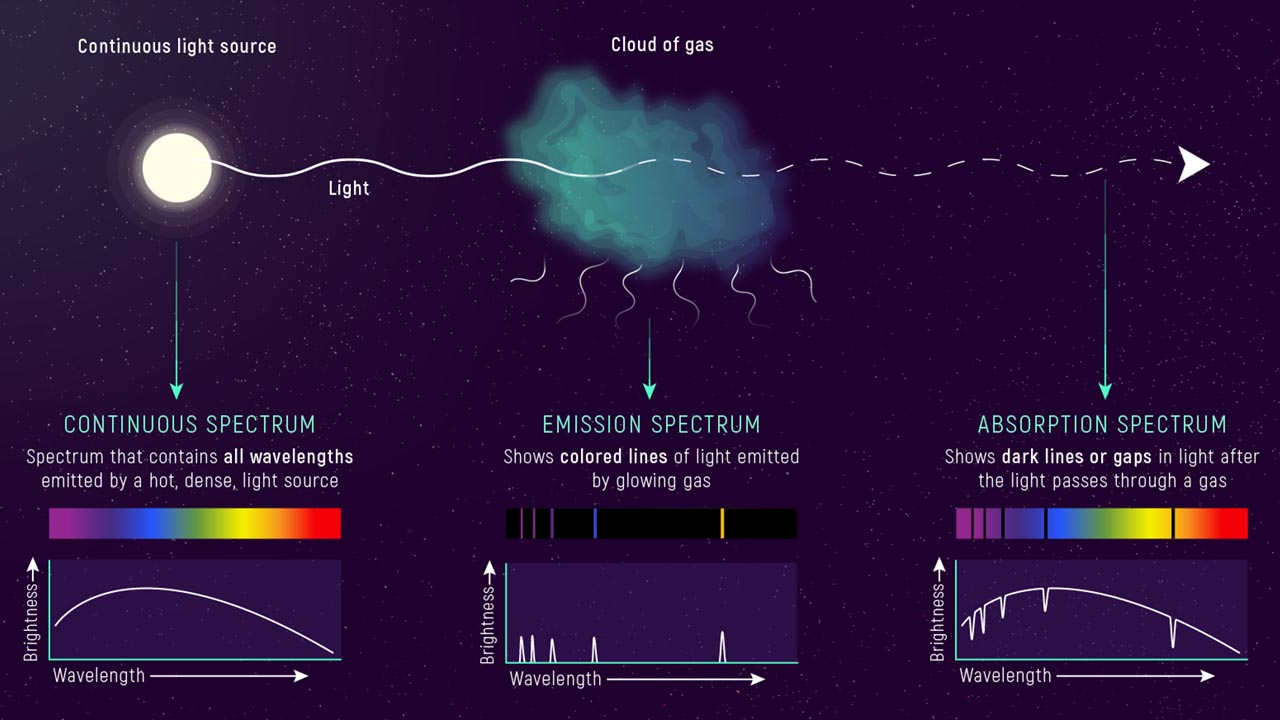
\includegraphics[width=\textwidth]{spectra.jpg}
    \caption{\centering \footnotesize{Types of Spectra: Continuous, Emission, Absorption \protect\cite{spectrapic}}}
    \label{fig:spectra}
\end{figure}

\subsubsection{What is 'Redshift'?}

\subsection{The Hubble Parameter} \label{sec:1.3}

\subsection{H and K Lines} \label{sec:1.4}

\subsection{More Terminology} \label{sec:1.5}

\section{The Procedure} 



\section{Results and Calculations}



\section{Conclusion}



\section{Applications of the Hubble Constant}




\newpage


%%%%%%%%%%%%%%%%%%%%%%%%%%%%%%%%%%%

\bibliographystyle{IEEEtran}
\bibliography{References}

\newpage

\section*{Appendix}
\addcontentsline{toc}{section}{Appendix}

\subsection*{Raw Data}
\addcontentsline{toc}{subsection}{Raw Data}

\listoffigures


\end{document}